\section{Transfer matrix model}
In general the transfer matrix method is good for simulating sandwich type structures where light is incident normal to the surface of a device. Examples of such devices are solar cells, optical filters or sensors. This method is good for understanding optical absorption, reflection and transition in these structures.  There are other more complex methods which can accomplish the same task such as FDTD, however general speaking the transfer matrix model will be orders of magnitude faster than these methods.

\subsection{The user interface}
The transfer matrix simulation tool can be reached from the \emph{Optical ribbon} in the main window by selecting \emph{Transfer matrix}.  If you click \emph{Run optical simulation} (see \ref{fig:transfermatrix0}) the distribution of light within the structure will be calculated as a function of position and wavelength. You can see from the top of the figure that there are various simulation modes. The full transfer matrix method is selected by selecting \emph{Transfer matrix}, this will do full optical simulation.  The other buttons represent other simplified approximations to the transfer matrix method that allow the user to explore more simple charge carrier generation profiles. From the left the push buttons in Figure \ref{fig:transfermatrix0} represent the following optical models:

\begin{itemize}
  \item \emph{Transfer matrix:} This is a full transfer matrix simulation that takes into account multiple reflections from the interfaces and optical loss within the structure. This is in effect solving the wave equation in 1D and is an accurate (and recommended) optical model to use. See section \ref{ssec:transfer_matrix_theory}. If you are unsure which model to pick, pick this one.

  \item \emph{Exponential profile}: This is a very simple optical model that assumes light decays exponentially according to the relation
\begin{equation}
I=I_{0}e^{-\alpha x}
\label{efield2}
\end{equation}
between layers and and assumes light is transmitted between layers according to the formula:
\begin{equation}
T=1.0-\frac{n_1-n_0}{n_1+n_0}
\label{equ:transfermatrixreflection}
\end{equation}
No reflection is accounted for.
  \item \emph{Flat profile}: The flat profile assumes light is constant within layers and only decreases at material interfaces according to equation \ref{equ:transfermatrixreflection}. One might want to use this model when trying to understand the charge carrier dynamics in a device but wants to remove the effects of a non-uniform charge generation generation profile.

  \item \emph{From file}: This can be used to import generation profiles from a file. It us generally used to import the results of more complex optical simulations such as those from external FDTD solvers.
  \item \emph{Constant value}: If you click on the arrow to the right of the simulation button you will be able to set the charge carrier generation rate within each layer by hand. Again this is generally used when trying to understand charge carrier dynamics or device performance without to consider a complex optical profile. This would allow one to plot graphs of charge generation rate v.s. $V_{oc}$ etc..
\end{itemize}

\begin{figure}[H]
\centering
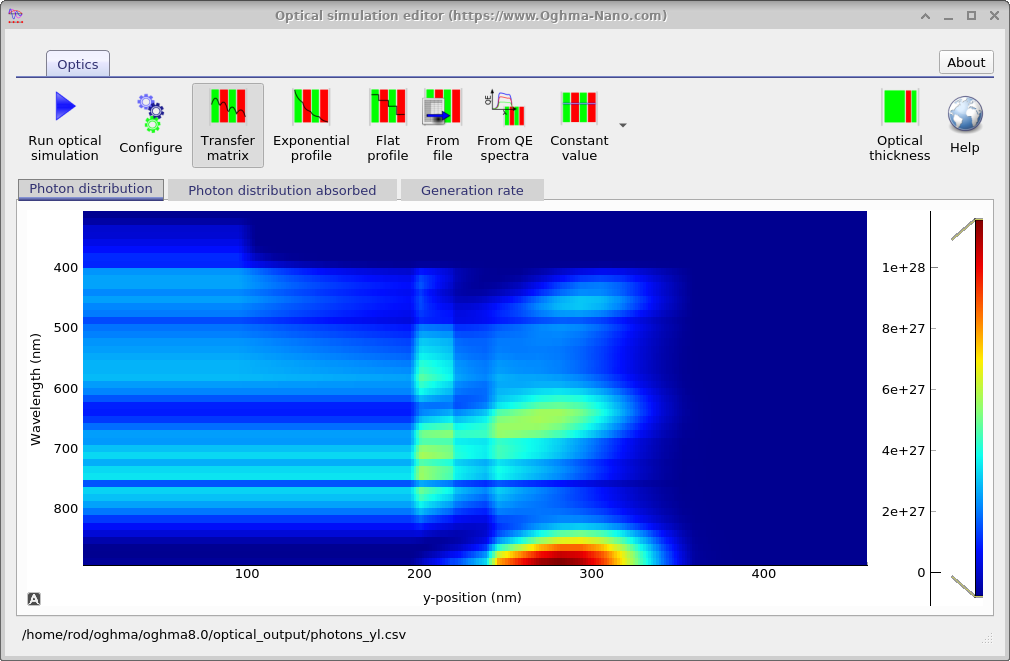
\includegraphics[width=1.0\textwidth,height=0.6\textwidth]{./images/transfer_matrix/opticalsimulation4.png}
\caption{This is the Transfer matrix optical simulation window, here you can view the photon density and the rate of photon absorption in the device.  The play button will run the simulation, exactly which flavour of transfer matrix simulation is run will depend on which push button you select from ribbon.}
\label{fig:transfermatrix0}
\end{figure}

The optical simulation window has various tabs which can be used to explore how light interacts with the device. These can be seen in figure \ref{fig:transfermatrix1}. The the top left image shows the photon density within the device, the image on the right shows the \emph{total} photon density within the layers of the device.  Notice how the reflection of the light of various layers causes interference patterns.  The image on the bottom left shows the configuration of the optical model. A key parameter that can be seen in this window is the \emph{Photon efficiency}, this parameter determines how many electron-hole pairs each photon that is absorbed within the active layer generates. In organic devices it accounts for geminate recombination, in other types of devices it should be set close to 1.0. Bottom right shows the same figure as in the top right of the figure, except by right clicking and playing with the menu options the figure has been converted into band diagram.  This can be useful for generating band diagram figures for papers.
  
\begin{figure}[H]
\centering
\begin{tabular}{ c c }

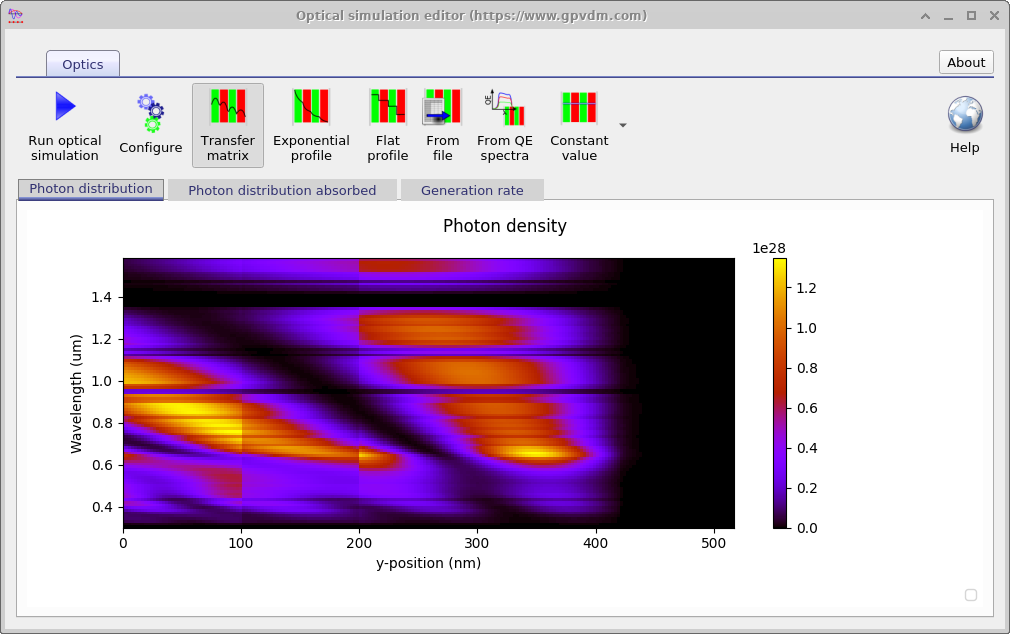
\includegraphics[width=0.5\textwidth,height=0.4\textwidth]{./images/transfer_matrix/opticalsimulation.png}

&
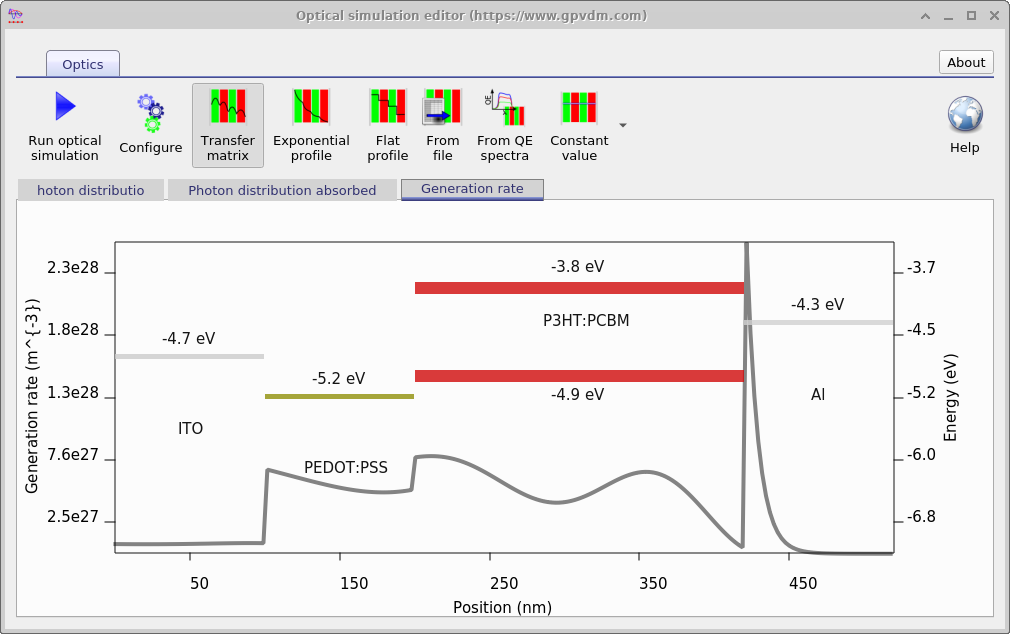
\includegraphics[width=0.5\textwidth,height=0.4\textwidth]{./images/transfer_matrix/opticalsimulation1.png}

\\
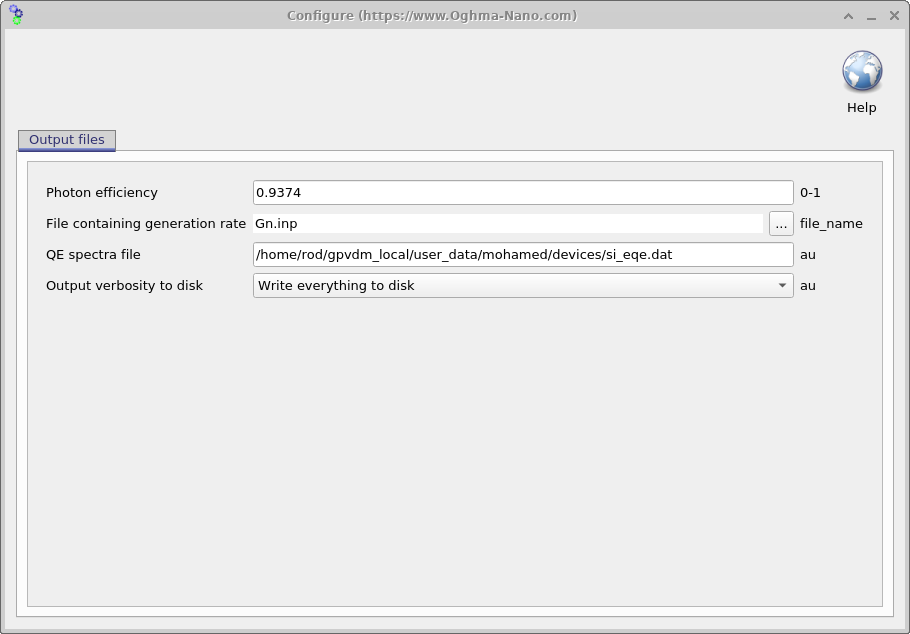
\includegraphics[width=0.5\textwidth,height=0.4\textwidth]{./images/transfer_matrix/opticalsimulation2.png}

&
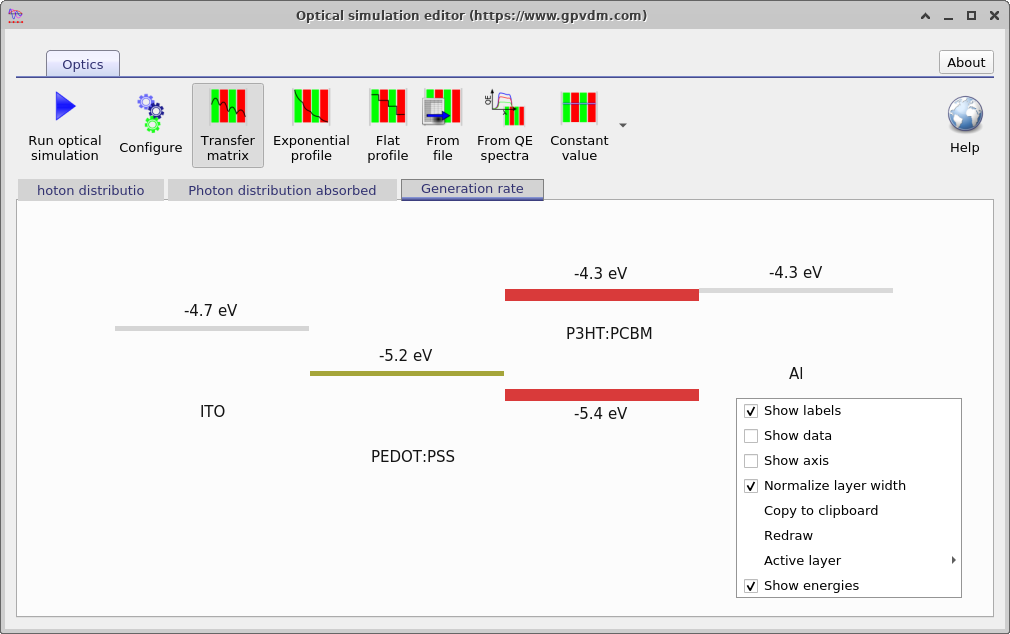
\includegraphics[width=0.5\textwidth,height=0.4\textwidth]{./images/transfer_matrix/opticalsimulation3.png}

\\
\end{tabular}
\caption{Various views of the optical simulation window}
\label{fig:transfermatrix1}
\end{figure}

\subsubsection{Running the transfer matrix simulation}
As described above, the transfer matrix simulation can be run by directly clicking on the play button.  However when running an electrical simulation the optical model is run automaticity without any user interaction. The only difference between the two ways of calling the optical simulation is that when the user directly calls the optical model more output files are written to disk, however when the optical simulation is run as part of an electrical simulation the number of files and output are limited as to not slow the electrical simulation. 
\newpage
\subsection{Output files}
After having run an optical simulation an overview of the results can be seen in the optical simulation window (Figure \ref{fig:transfermatrix0}) as described above. However more in depth information can be obtained from the \emph{Output} tab of the main window as shown in Figure \ref{fig:transfer_matrix_optical_output}.

\begin{figure}[H]
\centering
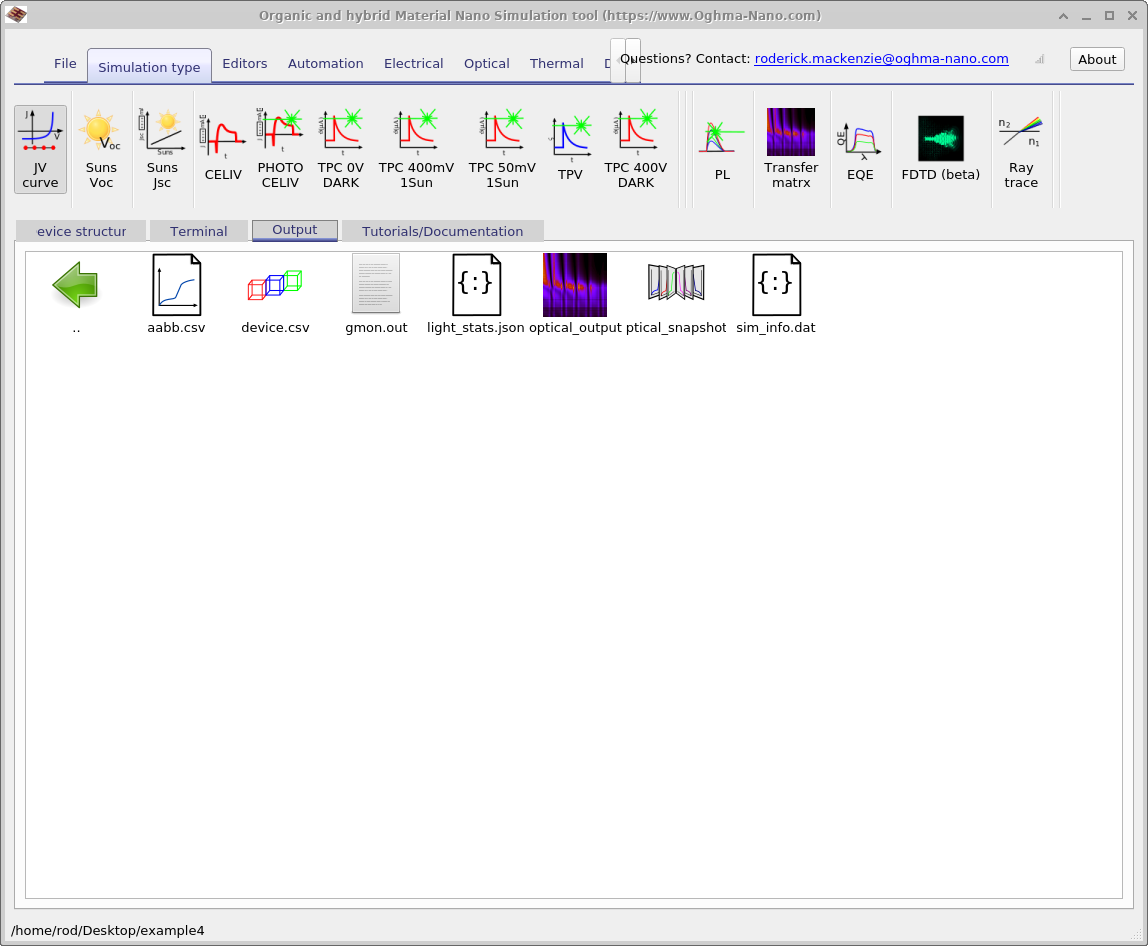
\includegraphics[height=0.6\textwidth,width=0.7\textwidth]{./images/transfer_matrix/optical_output.png}
\caption{The output tab shows the output from the transfer matrix simulation. Usually the optical\_output and optical\_snapshots files are only generated when the optical simulation is run directly and not as part of another simulation.}
\label{fig:transfer_matrix_optical_output}
\end{figure}

In Figure \ref{fig:transfer_matrix_optical_output} you can see two icons one called \emph{Optical output} and the other called \emph{optical\_snapshots} (in the figure it reads "ptica\_output" due to the text being hidden). If you double click on \emph{Optical output} it will bring up figure \ref{fig:transfermatrix0}. If you double click on \emph{optical\_snapshots} it will bring up Figure \ref{fig:transfer_matrix_optical_snapshots}. The optical snapshot window allows the user to view photon density, absorbed photons and electric field of the light. The information is displayed per wavelength so a detailed overview of device performance can be gained.


\begin{figure}[H]
\centering
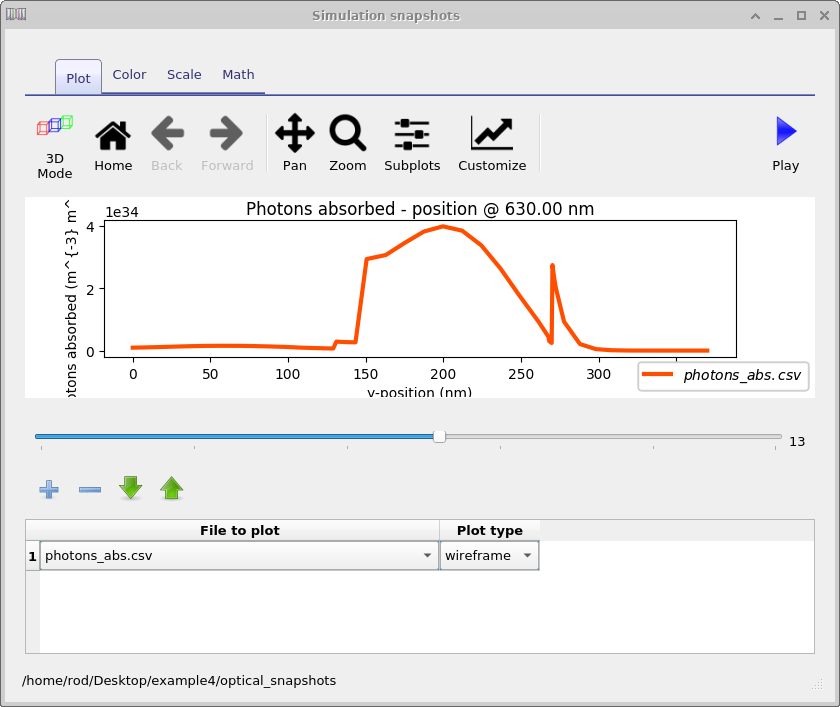
\includegraphics[height=0.6\textwidth,width=0.7\textwidth]{./images/transfer_matrix/optical_snapshots.png}
\caption{The optical snapshots window. This allows the user to view, Electric }
\label{fig:transfer_matrix_optical_snapshots}
\end{figure}

\subsubsection{The optical\_snapshots directory in depth}
The optical\_snapshots folder was described above and when accessed through the graphical interface allows the user to access photon density, absorbed photons and electric field of the light as a function of wavelength. However, it is simply a normal directory and the user can access it through a file explorer. If you open the directory using a tool such as windows explorer you will see something comparable to what is shown on the left of Figure \ref{fig:optical_snapshots_dir}. You can see folders numbered from 0 to 12 each folder represents a simulated wavelength. If you open a directory, say number 0, you will be presented with the files shown in the right hand of figure \ref{fig:optical_snapshots_dir}. These files contain the following information:

\begin{table}[H]
\begin{center}
\begin{tabular}{ |c|l|c| } 
 \hline
	File name 			& 	Description  \\ 
 \hline
	$alpha.csv$			&	y-position v.s. absorption @ given wavelength \\ 
	$data.json$			&	json file containing wavelength value \\ 
	$En.csv$ 			&	y-position (m) v.s. Electric field with -ve component (V/m)  @ given wavelength \\ 
	$Ep.csv$ 			&	y-position (m) v.s. Electric field with +ve component (V/m) @ given wavelength \\ 
	$G.csv$ 			&	y-position (m) v.s. Generation rate ($m^{-3} s^{-1}$)\\ 
	$n.csv$ 			&	y-position (m) v.s. Real part of the refractive index n (au) @ given wavelength\\ 
	$photons.csv$ 		&	y-position (m) v.s. photon density ($m^{-3}$) @ given wavelength \\ 
	$photons\_abs.csv$ 	&	y-position (m) v.s. photons absorbed ($m^{-3} s^{-1}$) @ given wavelength\\ 
 \hline
\end{tabular}
\caption{Files produced by the JV simulation}
\label{tab:jv_output}
\end{center}
\end{table}


\begin{figure}[H]
\centering
\begin{tabular}{ c c }

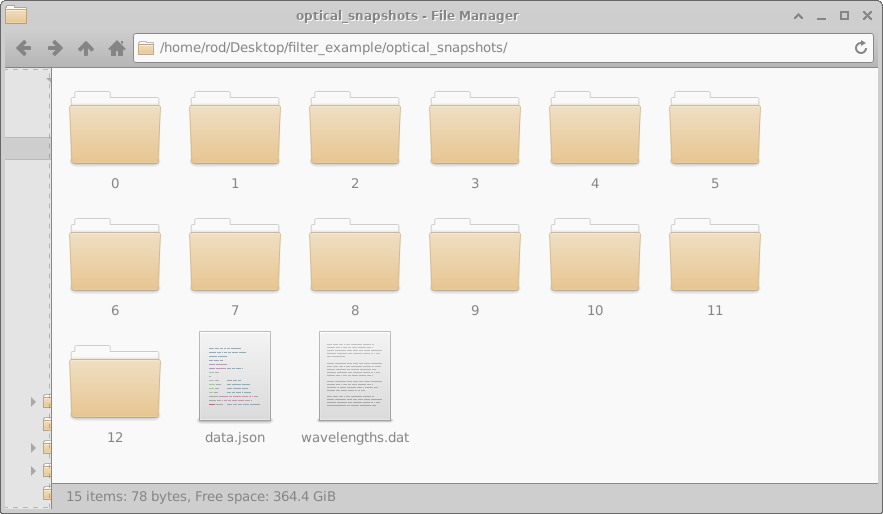
\includegraphics[width=0.5\textwidth,height=0.35\textwidth]{./images/transfer_matrix/snapshots_main_dir.png}

&
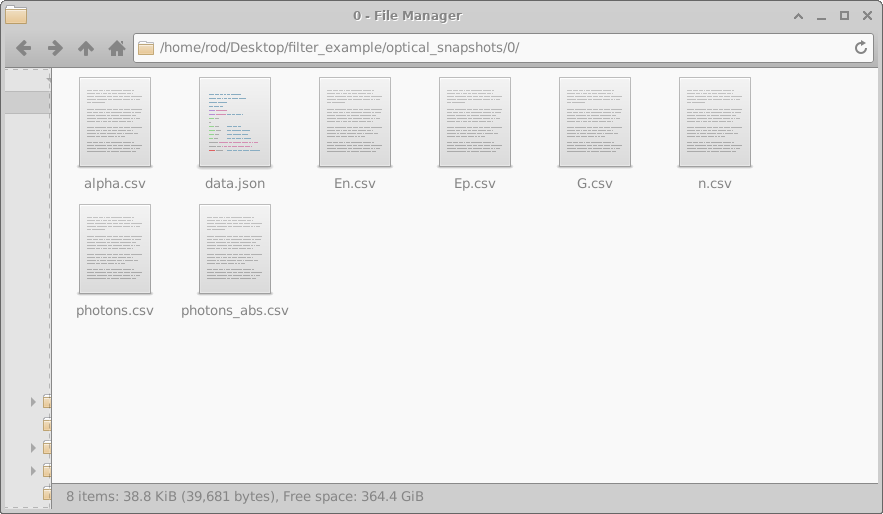
\includegraphics[width=0.5\textwidth,height=0.35\textwidth]{./images/transfer_matrix/snapshots_sub_dir.png}

\\
\end{tabular}
\caption{Various views of the optical simulation window}
\label{fig:optical_snapshots_dir}
\end{figure}

These files are simply plain text, if you open one it will look like \ref{fig:transfer_matrix_file_example}. The first line of this file contains some information about the content of the file to help with plotting. The second line tells the user what the x and y axis contain then the following lines contain the data.

\begin{figure}[H]
\centering
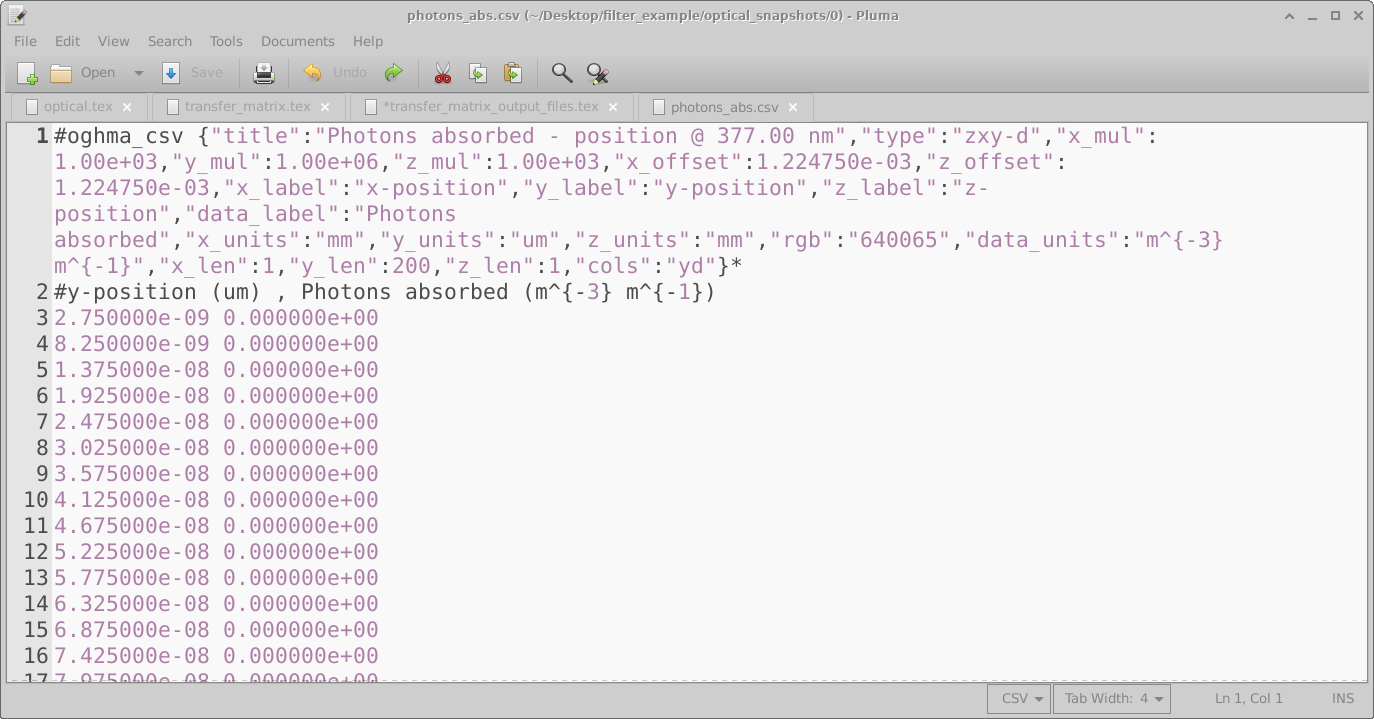
\includegraphics[height=0.5\textwidth,width=0.7\textwidth]{./images/transfer_matrix/snapshots_file_example.png}
\caption{The content of photons\_abs.csv.}
\label{fig:transfer_matrix_file_example}
\end{figure}

\subsubsection{The optical\_output folder in depth}
While the optical\_snapshots directory allows data to be plotted per simulated wavelength, the optical\_output gives 2D maps of wavelength v.s. position for various simulation parameters. The content of the directory is shown in figure \ref{fig:optical_output_directory}.

\begin{figure}[H]
\centering
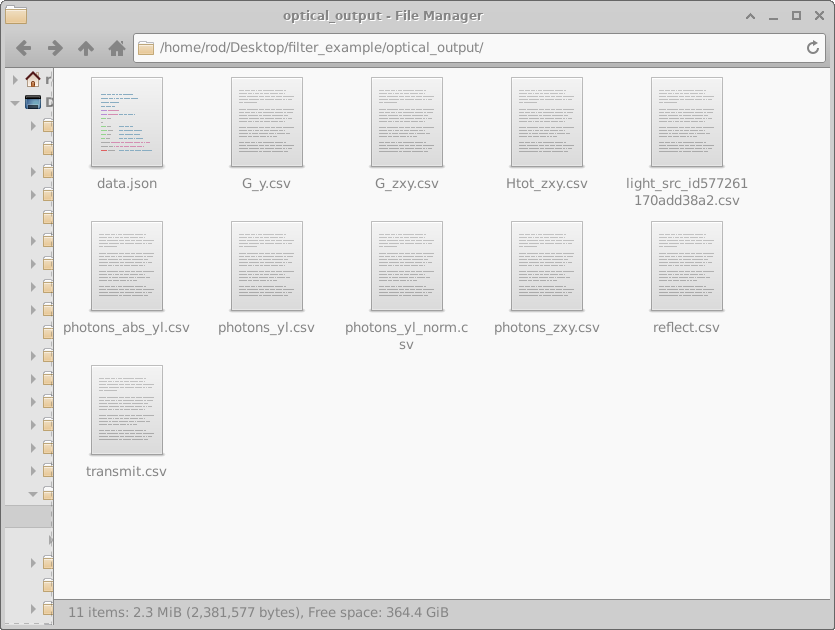
\includegraphics[height=0.5\textwidth,width=0.7\textwidth]{./images/transfer_matrix/optical_output_dir.png}
\caption{The content of optical\_output directory}
\label{fig:optical_output_directory}
\end{figure}

The files shown in Figure \ref{fig:optical_output_directory} are described in table \ref{tab:optical_output_files}.

\begin{table}[H]
\begin{center}
\begin{tabular}{ |c|l|c| } 
 \hline
	File name 				& 	Description  & Plot type\\ 
 \hline
	data.json				&	Miscellaneous simulation information in json format			&	1D \\
 	G\_y.csv				&	y-position (m) v.s. Charge generation rate ($m^{-3} s^{-1}$)&	2D \\
	G\_zxy.csv				&	zxy-position (m) v.s. Charge generation rate ($m^{-3} s^{-1}$)	&	2D \\
 	Htot\_zxy.csv			&	zxy-position (m) v.s. Optical heat generation ($W m^{-3}$)	&	2D \\
 	light\_src\_id\_xxx.csv	&	wavelength (m) v.s. Light intensity from source ($W/m$)		&	2D \\
 	photons\_abs\_yl.csv	&	wavelength (m) v.s. y-position (m) v.s. photons absorbed ($m^{-3} s^{-1}$)	&	2D \\
 	photons\_yl.csv			&	wavelength (m) v.s. y-position (m) v.s. Photon density ($m^{-3} s^{-1}$)&	2D\\
 	photons\_yl\_norm.csv	&	wavelength (m) v.s. y-position (m) v.s. Normalized photons (au)&	2D \\
 	reflect.csv				&	wavelength (m) v.s. Light reflected from the stack 	&	1D  \\
 	transmit.csv			&	wavelength (m) v.s. Transmitted though the stack	&	1D  \\
 \hline
\end{tabular}
\caption{Files produced by the JV simulation}
\label{tab:optical_output_files}
\end{center}
\end{table}

\newpage



\subsection{Simulating optically thick layers (incoherent layers)}
Typical optoelectronic devices have layer thicknesses between 10 nm and 100 nm.  However often these devices are deposited on top of substrates that are between 10 mm and 1 cm thick and often one wants to not only simulate the device but also the impact of the substrate. Thus to perform this type of simulation one will need a simulation tool that covers length scales from the nm top the meter scale. There are three problems with doing this:

\begin{itemize}
  \item Problem 1: \emph{Simulating different length scales}: Computers don't like doing maths with numbers that are very big and small very often this results in large computational/rounding errors, there is more on this in secton \ref{ssec:big_small_numbers}.
  \item Problem 2: \emph{The wavelength of light}: The wavelength of light is far smaller than 1 cm thus to get sensible answers out of the simulation one will need a very large number of mesh points correctly represent the constructive/negative interference of the light within the layer.
  \item Problem 3: \emph{The light will not be coherent}: The transfer matrix model assumes light comes from a single direction at 90 degrees to the interface and there are no defects in the material. For a thick layer this will not be true. 
\end{itemize}

To get around these issues OghmaNano uses two strategies. The first is to give the user the option to only consider absorption and neglect phase changes within a layer, to form a so called incoherent layer (this solves problem 2 and 3). This can be selected from the layer editor in the main window see Figure \ref{fig:transfer_matrix_layer_editor}. Notice in the column entitled \emph{Solve optical problem}, the first two layers (air and glass) have \emph{Yes - k} selected, and the other layers have \emph{Yes - n/k} selected. This means that in layers with \emph{Yes - n/k} phase changes of the light will be considered but in the layers marked \emph{Yes - k} only attenuation losses will be accounted for and thus it can be thought of as an incoherent layer.

\begin{figure}[H]
\centering
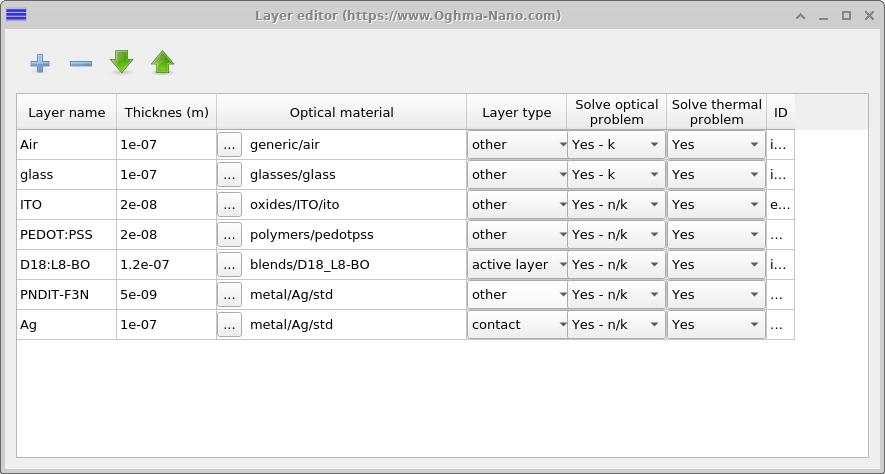
\includegraphics[width=0.8\textwidth,height=0.5\textwidth]{./images/transfer_matrix/layer_editor.png}
\caption{The layer editor showing both \emph{coherent layers} and \emph{incoherent layers}}
\label{fig:transfer_matrix_layer_editor}
\end{figure}

To get around the problem of having to simulate different length scales (problem 1) OghmaNano allows the user to set an \emph{effective} optical depth for any layer.  So one can for example setup a layer in the layer editor of width 100 nm, but set it's \emph{effective} depth to a much larger value such as 1 m. This works by multiplying the absorption coefficient of the layer by the ratio:

\begin{equation}
\alpha_{effective}(\lambda)=\alpha(\lambda) \frac{L_{effective}}{L_{simulation}}
\label{effective_depth}
\end{equation}

Where $\alpha_{effective}$ is the effective absorption used in the simulation, $\alpha$ is the true value of absorption for the material, $L_{effective}$ is the effective layer thickness (say 1 m or 1 km), and $L_{simulation}$ is the thickness of the layer in the simulation window. Not only does this approach reduce numerical issues (problem 1) but it also allows the user to plot meaningful graphs of the simulation results, without most of the plot taken up by the substrate and the device only appearing as a tiny slither on the edge of the graph.

If you want to use this feature, then set up a device structure as shown in \ref{fig:transfer_matrix_layer_editor} then in the transfer matrix window click the Optical Thickness button (top right of Figure \ref{fig:optical_thickness}). Then the window \ref{fig:optical_thickness_window} will appear. In this window you can set the \emph{effective optical thickness} of any layer. In this case we have set the glass to be 1 meter thick.

\begin{minipage}{0.5\textwidth}
	\centering
	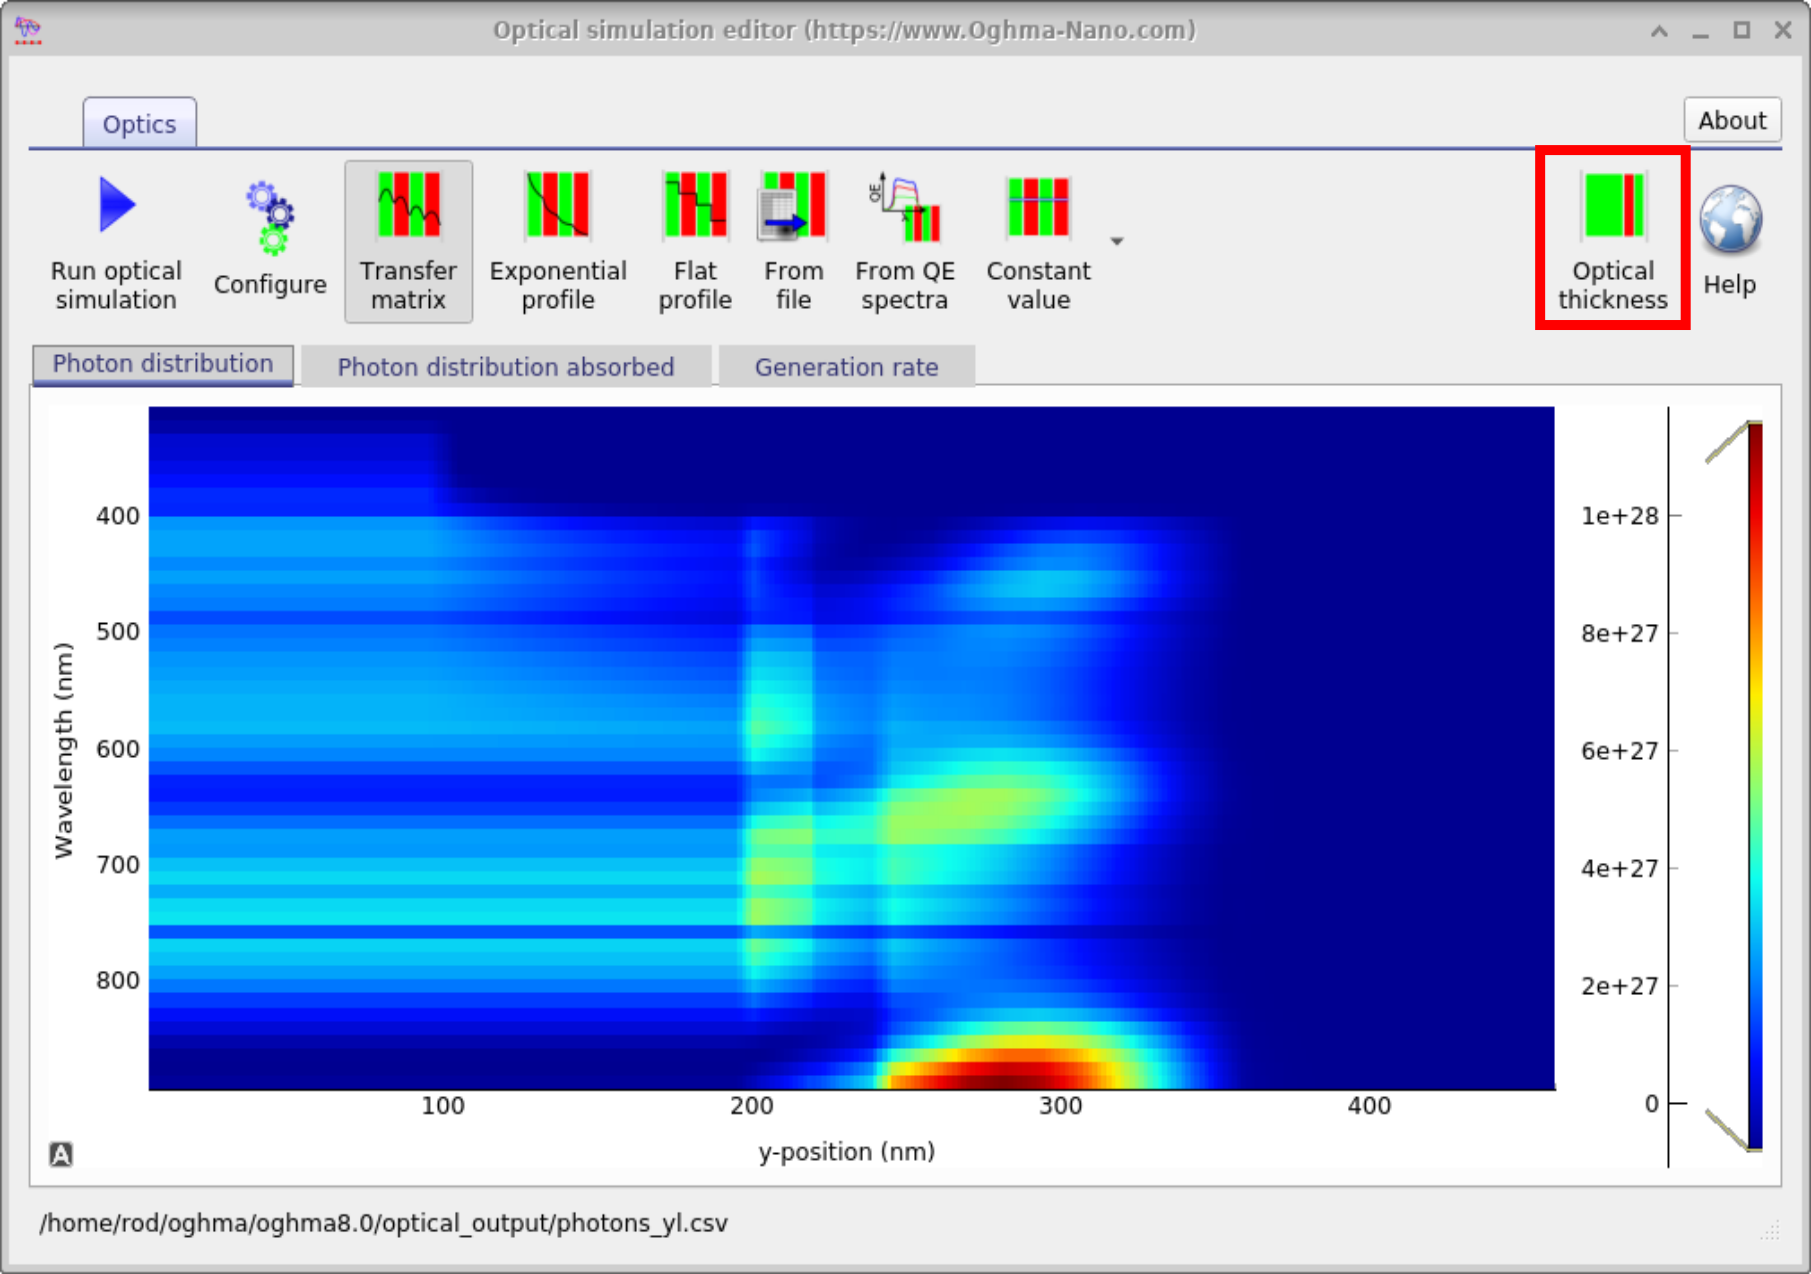
\includegraphics[width=\linewidth,height=0.8\linewidth]{./images/transfer_matrix/thickness.png}
	\captionof{figure}{Opening the effective optical thickness window.}
	\label{fig:optical_thickness}
\end{minipage}
\hspace{4pt}
\begin{minipage}[]{0.5\linewidth}
	\centering
	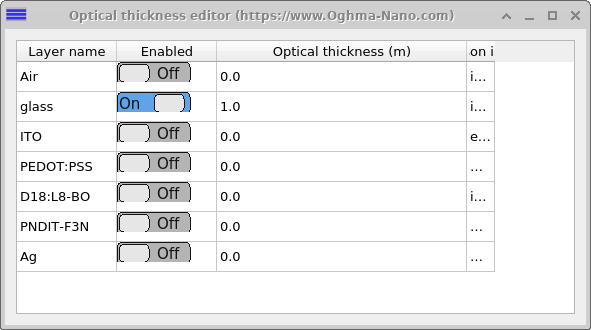
\includegraphics[width=\linewidth,height=0.6\linewidth]{./images/transfer_matrix/layer_thickness.png}
	\captionof{figure}{The effective optical thickness window, you can see that for this structure the optical thickness of glass has been set to 1 meter.}
	\label{fig:optical_thickness_window}
\end{minipage}


\pagebreak

\subsection{Theory of the transfer matrix method}  \label{ssec:transfer_matrix_theory}
On the left of the interface the electric field is given by

\begin{equation}
E_{1}=E^{+}_{1} e^{-j k_1 z}+E^{-}_{1} e^{j k_1 z}
\label{efield1}
\end{equation}
and on the right hand side of the interface the electric field is given by
\begin{equation}
E_{2}=E^{+}_{2} e^{-j k_2 z}+E^{-}_{2} e^{j k_2 z}
\label{efield2}
\end{equation}

Maxwel's equations give us the relationship between the electric and magnetic fields for a plane wave.

\begin{equation}
\nabla \times E=-j\omega \mu H 
\end{equation}
which simplifies to:
\begin{equation}
\frac{\partial E} {\partial z}=-j\omega \mu H 
\label{maxwel}
\end{equation}

Applying equation \ref{maxwel} to equations \ref{efield1}-\ref{efield2}, we can get the magnetic field on the left of the interface
\begin{equation}
-j \mu \omega H^{y}_{1}=-j k_1 E^{+}_{1} e^{-j k_1 z}+j k_1 E^{-}_{1} e^{j k_1 z}
\end{equation}
and on the right of the interface
\begin{equation}
-j \mu \omega H^{y}_{2}=-j k_2 E^{+}_{2} e^{-j k_2 z}+j k_2 E^{-}_{2} e^{j k_2 z}.
\end{equation}

Tidying up gives,
\begin{equation}
H^{y}_{1}=\frac{k}{\omega \mu}E^{+}_{1} e^{-j k_1 z}-\frac{k}{\omega \mu} E^{-}_{1} e^{j k_1 z}
\end{equation}

\begin{equation}
H^{y}_{2}=\frac{k}{\omega \mu}E^{+}_{2} e^{-j k_2 z}-\frac{k}{\omega \mu} E^{-}_{2} e^{j k_2 z}
\end{equation}

%%%%%%%%%%%
\subsubsection{Boundary conditions}
We now apply the electric and magnetic boundary conditions\cite{0953-8984-25-21-215301}
\begin{equation}
\mathbf{n} \times (\mathbf{E_2}-\mathbf{E_1})=0
\end{equation}

\begin{equation}
\mathbf{n} \times (\mathbf{H_2}-\mathbf{H_1})=0
\end{equation}

We let the interface be at z=0, which gives,
\begin{equation}
(E_{2}^{+}+E_{2}^{-})-(E_{1}^{+}+E_{1}^{-})=0
\label{electric_boundary}
\end{equation}
and
\begin{equation}
\frac{k_1}{\omega \mu}(E_{2}^{+}-E_{2}^{-})-(E_{1}^{+}-E_{1}^{-})\frac{k_2}{\omega \mu}=0
\end{equation}
.
The wavevector is given by
\begin{equation}
k=\frac{2 \omega }{\lambda}=\frac{\omega n}{c}
\end{equation}
.
We can therefore write the magnetic boundary condition as
\begin{equation}
n_2 (E_{2}^{+}-E_{2}^{-}) - n_1 (E_{1}^{+}-E_{1}^{-})=0
\label{mag_boundary}
\end{equation}

\subsubsection{Forward propagating wave}
Rearrange equation, \ref{mag_boundary} to give,

\begin{equation}
E_{1}^{-} = E_{1}^{+}-\frac{n_2}{n_1}(E_{2}^{+}-E_{2}^{-})
\end{equation}
Inserting in equation \ref{electric_boundary}, gives 
\begin{equation}
E_{2}^{+}+E_{2}^{-}=E_{1}^{+}+E_{1}^{+}-\frac{n_2}{n_1}(E_{2}^{+}-E_{2}^{-})
\end{equation}

\begin{equation}
2E_{1}^{+}=E_{2}^{+}+E_{2}^{-}+\frac{n_2}{n_1}(E_{2}^{+}-E_{2}^{-})
\end{equation}

\begin{equation}
2E_{1}^{+}\frac{n_1}{n_1+n_2}=E_{2}^{+}+E_{2}^{-}\frac{n_1-n_2}{n_1+n_2}
\end{equation}

\subsubsection{Backwards propagating wave}
Rearrange equation, \ref{mag_boundary} to give,

\begin{equation}
E_{1}^{+}=E_{1}^{-} +\frac{n_2}{n_1}(E_{2}^{+}-E_{2}^{-})
\end{equation}

Inserting in equation \ref{electric_boundary}, gives 
\begin{equation}
E_{2}^{+}+E_{2}^{-}=E_{1}^{-} +\frac{n_2}{n_1}(E_{2}^{+}-E_{2}^{-})+E_{1}^{-}
\end{equation}

\begin{equation}
2E_{1}^{-}=E_{2}^{+}+E_{2}^{-}- \frac{n_2}{n_1}(E_{2}^{+}-E_{2}^{-})
\end{equation}

\begin{equation}
2E_{1}^{-}\frac{n_1}{n_1+n_2}=E_{2}^{+}\frac{n_1-n_2}{n_1+n_2}+E_{2}^{-}
\end{equation}
Which is the same result as obtained in \cite{10.1063/1.1534621}.

These equations become:

\begin{equation}
E_{1}^{-}t_{12}=E_{2}^{+}r_{12}+E_{2}^{-}
\end{equation}

and
\begin{equation}
E_{1}^{+}t_{12}=E_{2}^{+}+E_{2}^{-}r_{12}
\end{equation}

Accounting for propagation we can write.  Note the change in sign between \cite{10.1063/1.1534621} and this work, this is because of how I have defined my wave equation. 
\begin{equation}
E_{1}^{+}t_{12}=E_{2}^{+}e^{\zeta_2 d_1}+E_{2}^{-}r_{12}e^{-\zeta_2 d_1}
\end{equation}
and

\begin{equation}
E_{1}^{-}t_{12}=E_{2}^{+}r_{12}e^{\zeta_2 d_1}+E_{2}^{-}e^{-\zeta_2 d_1}
\end{equation}

where
\begin{equation}
\zeta=\frac{2\pi}{\lambda} \bar{n}
\end{equation}

%Note that in  \cite{10.1063/1.1534621} they use $\zeta_1$ instead of $\zeta_2$.  This is a mistake and makes a difference at interfaces.
For a device with non reflecting back contacts:

$
 \begin{pmatrix}
  e^{\zeta d}         & 0                   & 0                  & 0                   &r_{01}e^{-\zeta d}     & 0                       & 0                    & 0   \\
  -t_{12}              & e^{\zeta d}        & 0                  & 0                   &0                     & r_{12}e^{-\zeta d}      & 0                   & 0    \\
  0                    & -t_{23}             & e^{\zeta d}       & 0			&0                     & 0                      & r_{23}e^{-\zeta d}   & 0    \\
  0                    & 0                   & -t_{34}            & e^{\zeta d}	& 0			& 0                      & 0                   & r_{34}e^{-\zeta d} \\
  0                    &r_{12}e^{\zeta d_1} & 0                   & 0                  & -t_{12}			&e^{-\zeta d}           & 0                      & 0       \\
  0                    &0                    & r_{23}e^{\zeta d}  & 0                  & 0                     	   &-t_{23}                & e^{-\zeta d}           & 0    \\
  0                    &0                    & 0                   & r_{34}e^{\zeta d} & 0     			   &0                     & -t_{34}                & e^{-\zeta d}    \\
  0                    &0                    & 0                   & 0		  	& 0				   &0                     & 0			   & -t_{45}        \\
 \end{pmatrix}
\begin{pmatrix}
  E_{1}^{+} \\
  E_{2}^{+} \\
  E_{3}^{+}  \\
  E_{4}^{+} \\
  E_{1}^{-} \\
  E_{2}^{-} \\
  E_{3}^{-}  \\
  E_{4}^{-}  \\
 \end{pmatrix}
=
\begin{pmatrix}
  t_{01}E_{external} \\
  0 \\
  0 \\
  0 \\
  0 \\
  0 
 \end{pmatrix}
$



\subsection{Refractive index and absorption}
\begin{equation}
E(z,t)=Re(E_0 e^{j(-kz+\omega t)})= Re(E_0 e^{j(\frac{-2 \pi (n+j\kappa)}{\lambda}z + \omega t)})=e^{\frac{2\pi\kappa z}{\lambda}}Re(E_0 e^{\frac{j(-2 \pi (n+j\kappa)}{\lambda}z +\omega t})
\end{equation}
And because the intensity is proportional to the square of the electric field the absorption coefficient becomes

\begin{equation}
e^{-\alpha x}=e^{\frac{2\pi\kappa z}{\lambda}}
\end{equation}

\begin{equation}
\alpha=-\frac{4\pi\kappa}{\lambda_0}
\end{equation}


\newpage
\vfill


